\documentclass[12pt,fleqn]{article}

\usepackage[utf8]{inputenc}
\usepackage[T2A]{fontenc}
\usepackage{amssymb,amsmath,mathrsfs,amsthm}
\usepackage[russian]{babel}
\usepackage[pdftex]{graphicx}
\usepackage{multirow}
\usepackage{indentfirst}
\usepackage[colorlinks,linkcolor=blue(ryb),citecolor=blue(ryb), unicode]{hyperref}

\usepackage{xcolor}
\usepackage{sectsty}

\usepackage{amsmath}
\usepackage{systeme}
\definecolor{blue(ryb)}{rgb}{0.2, 0.2, 0.6}

\usepackage{listings}
\usepackage{xcolor}

\definecolor{codegreen}{rgb}{0,0.6,0}
\definecolor{codegray}{rgb}{0.5,0.5,0.5}
\definecolor{codepurple}{rgb}{0.58,0,0.82}
\definecolor{backcolour}{rgb}{0.95,0.95,0.92}

\lstdefinestyle{mystyle}{
    backgroundcolor=\color{backcolour},   
    commentstyle=\color{codegreen},
    keywordstyle=\color{magenta},
    numberstyle=\tiny\color{codegray},
    stringstyle=\color{codepurple},
    basicstyle=\ttfamily\footnotesize,
    breakatwhitespace=false,         
    breaklines=true,                 
    captionpos=b,                    
    keepspaces=true,                 
    numbers=left,                    
    numbersep=5pt,                  
    showspaces=false,                
    showstringspaces=false,
    showtabs=false,                  
    tabsize=2
}

\lstset{style=mystyle}


%\usepackage[ruled,section]{algorithm}
%\usepackage[noend]{algorithmic}
%\usepackage[all]{xy}

% Параметры страницы
\sectionfont{\color{blue(ryb)}}
\subsubsectionfont{\color{blue(ryb)}}
\subsectionfont{\color{blue(ryb)}}
\textheight=24cm % высота текста
\textwidth=16cm % ширина текста
\oddsidemargin=0pt % отступ от левого края
\topmargin=-2.5cm % отступ от верхнего края
\parindent=24pt % абзацный отступ
\parskip=0pt % интервал между абзацам
\tolerance=2000 % терпимость к "жидким" строкам
\flushbottom % выравнивание высоты страниц
%\def\baselinestretch{1.5}
\setcounter{secnumdepth}{0}
\renewcommand{\baselinestretch}{1.1}

\newcommand{\norm}{\mathop{\rm norm}\limits}
\newcommand{\real}{\mathbb{R}}

\newcommand{\ex}{\mathbb{E}}
\newcommand{\diag}{\mathrm{diag}}
\newcommand{\intset}{\mathrm{int}}
\newcommand{\softmax}{\mathop{\rm softmax}\limits}
\newcommand{\lossfunc}{\mathcal{L}'}
\newcommand{\elbo}{\mathcal{L}}
\newcommand{\normal}[3]{\mathcal{N}(#1 | #2, #3)}
\newcommand{\dd}[2]{\frac{\partial#1}{\partial#2}}
\newcommand{\kl}[2]{\mathop{KL}(#1 \parallel #2)}
\newcommand{\nm}{\mathcal{N}}
\newcommand{\sle}{\; \Rightarrow \;}
\newcommand{\indpos}{\mathbf{I}_{d_k}^{+}[i, j]}
\newcommand{\indneg}{\mathbf{I}_{d_k}^{-}[i, j]}

\usepackage{pgfplots}

%my settings
\graphicspath{{../_figures/}}
\usepackage{wrapfig}
\usepackage[font=small]{caption}
\usepackage{multirow}

\title{Композиции алгоритмов для решения задачи регрессии}

\author{Тыцкий Владислав}
\date{Декабрь 2020}

\begin{document}

\maketitle

\section{1. Введение}
В данном отчете исследуется поведение алгоритмов Random Forest и Gradient Boosting
на примере датасета стоимости квартир, где целевая переменная это цена квартиры.

Датасет был разделен на обучающую и тестирующую выборки. Объекты имеют много категориальных
признаков, но было решено не использовать One Hot Encoding в виду 
специфики алгоритмов RF и GB --- Оба алгоритма работают над деревьями, поэтому
''категоризация'' числовых величин(хотя на деле их необходимо считать категориальными)
может происходить путем построения более глубоких деревьев. Да, GB строит неглубокие деревья,
но так как каждый следующий алгоритм старается исправить ошибки уже построенной композиции,
то признак тоже может ''категоризироваться''.\footnote{Под категоризацией признака
подразумевается то, что алгоритм ''не вводит'' на нем отношение порядка.}

\section{2. Random Forest}
Random Forest --- это композиционный алгоритм машинного обучения над деревьями. 
Каждое дерево вносит одинаковый вклад в итоговый прогноз и строится независимо. Обычно для обучения 
очередного дерева используют
бэггинг для генерации обучающих выборок. Это уменьшает скорреллированность алгоритмов
, а значит и разброс всей композиции. Кроме того можно генерировать случайную подвыборку
признаков и обучать алгоритм только на этих признаках. Такой подход тоже может уменьшать
скоррелированность алгоритмов.

\newpage 

\subsection{2.1. Зависимость ошибки от количества признаков}

\begin{figure}[htb]
    \centering
    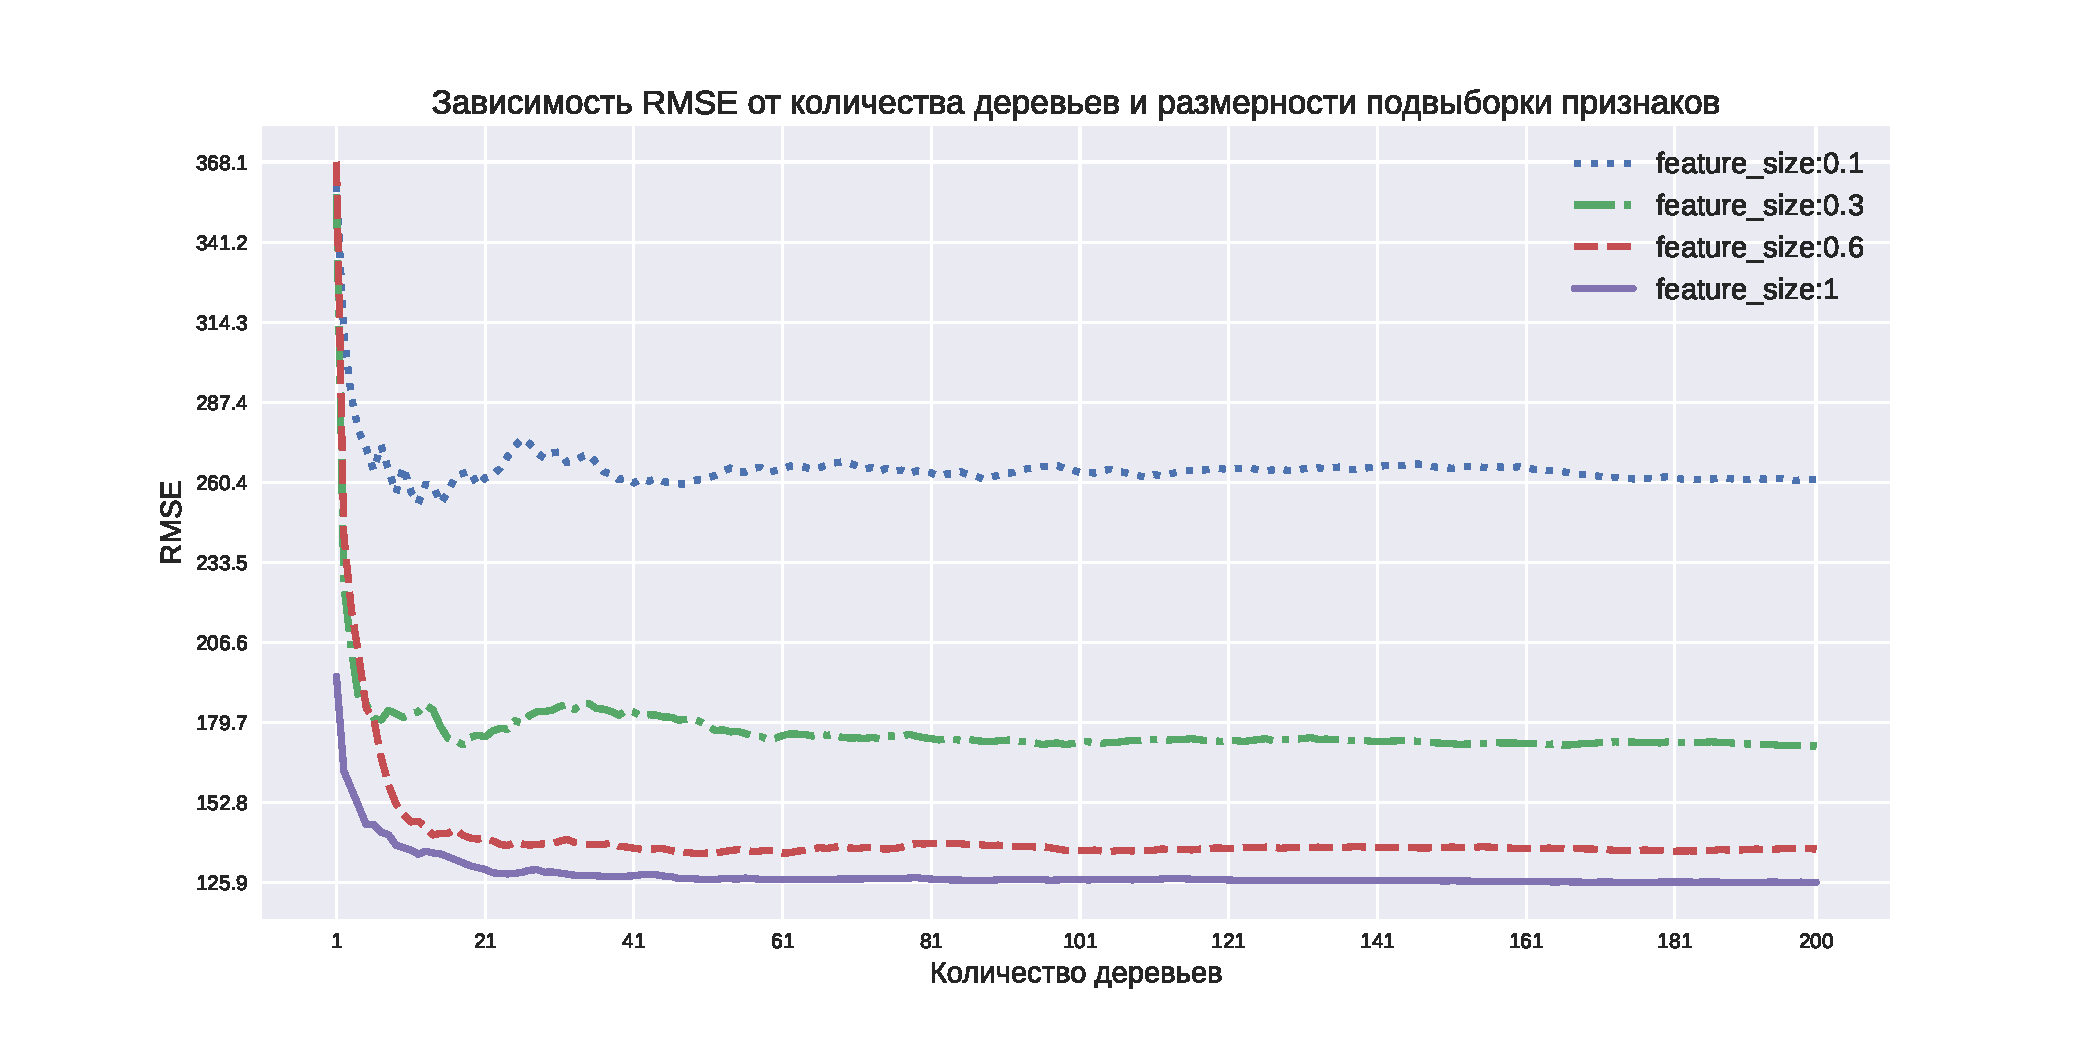
\includegraphics[width=15cm]{21.pdf}
    \caption{Влияние размерности подвыборки на RMSE}
    \label{feature_size_RF}
\end{figure}

На Рис. \ref{feature_size_RF} видно, что лучшее качество получается
при полном наборе признаков для любого количества деревьев в композиции.
Отметим, что чем больше feature\_size, тем лучше качество для данного датасета.
Также можно отметить, что качество перестает расти где-то после 60-ого 
дерева в композиции.

\subsection{2.2. Зависимость ошибки от количества и глубины деревьев}
\begin{figure}[htb]
    \centering
    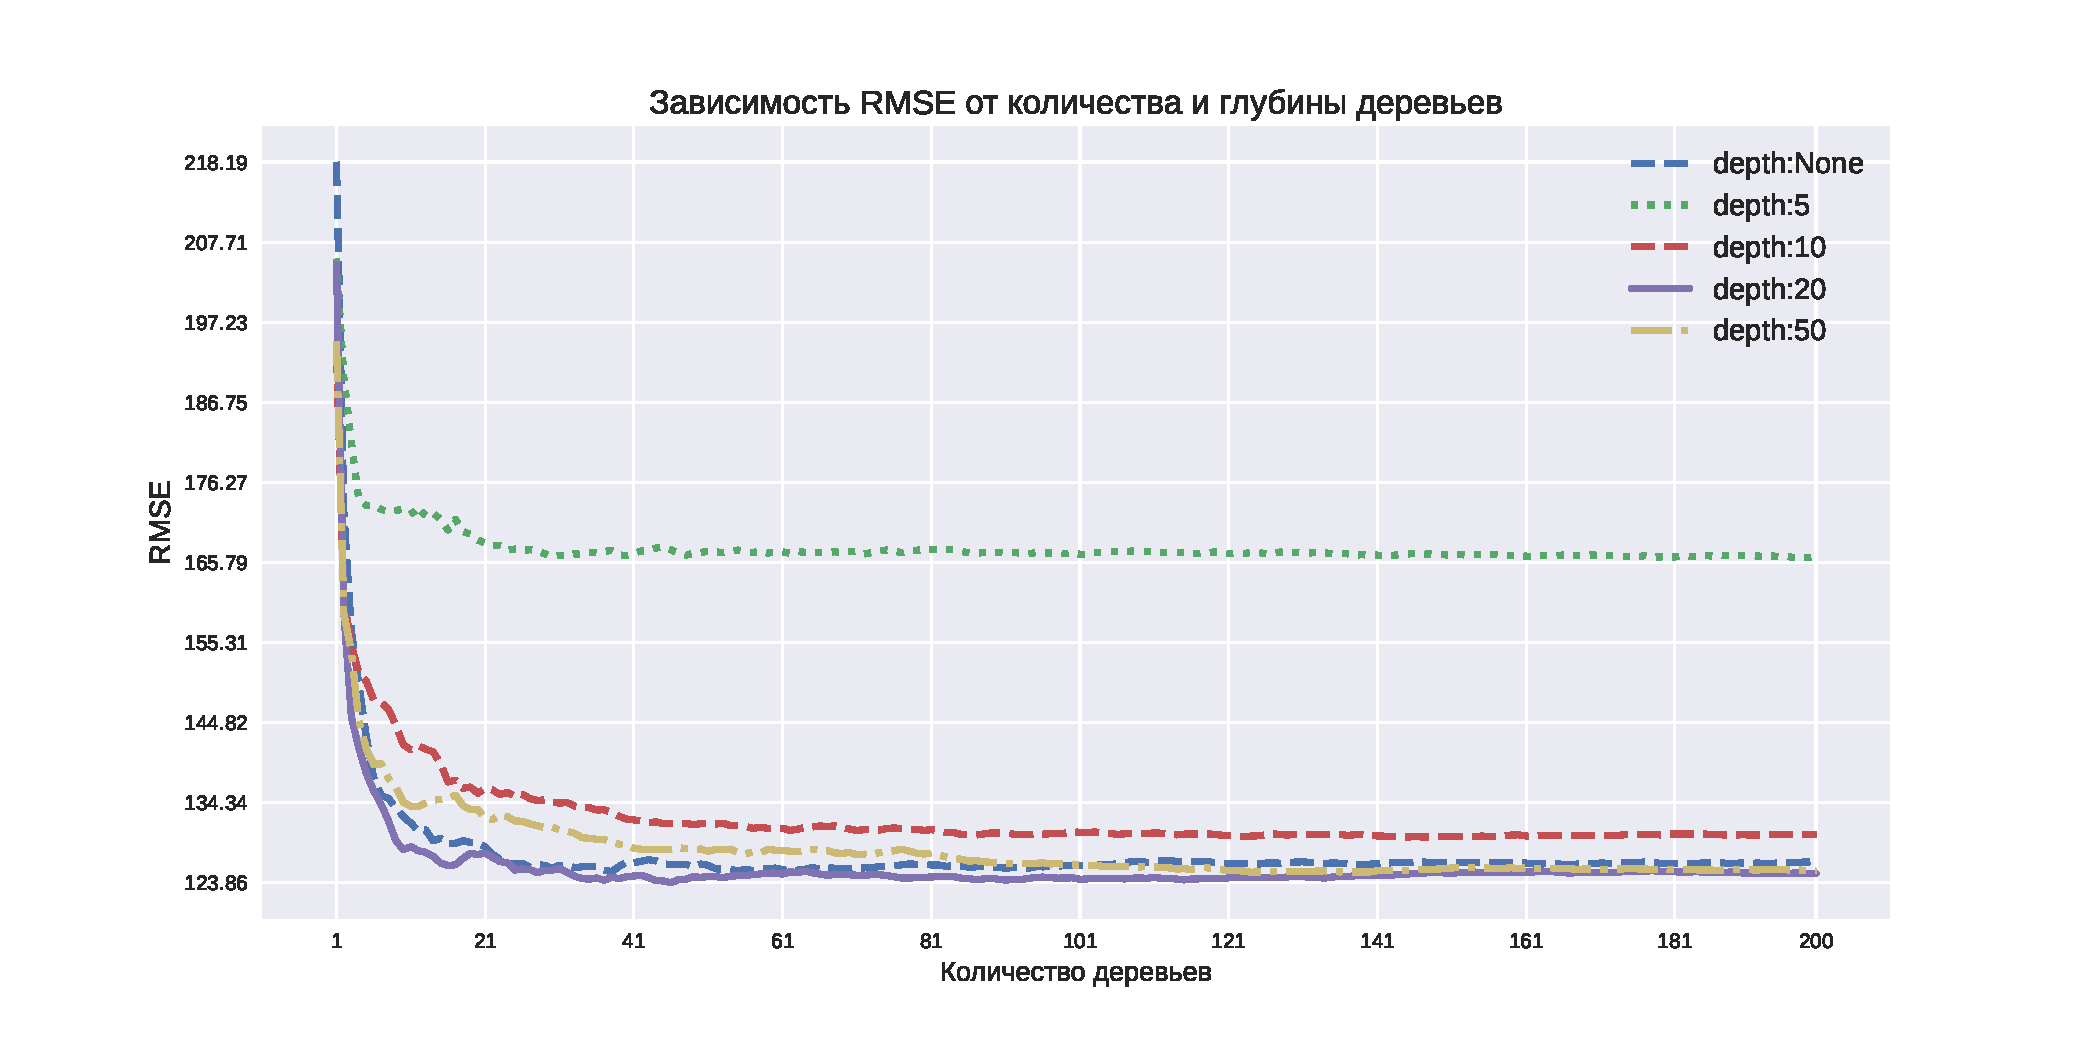
\includegraphics[width=15cm]{22.pdf}
    \caption{Влияние глубины деревьев в композиции}
    \label{depth_RF}
\end{figure}

Важным параметром при обучении алгоритма Random Forest является максимальная
глубина деревьев в композиции. Если максимальная глубина мала, то деревья
недообучатся и смещение композиции будет большим, если глубина большая, то может
возникнуть риск переобучения(большой разброс), но в случае RF такое происходит нечасто
т.к. вся идея алгоритма в том, чтобы строить слабо коррелированные переобученные деревья и 
составлять из них композицию, тем самым уменьшая разброс.

На Рис. \ref{depth_RF} видно, что деревья без ограничений на глубину\footnote{detph: None}
имеют, хоть и немного, большую ошибку, чем деревья с ограничением на глубину 20, 50. Как и 
ожидалось деревья с маленькой максимальной глубиной имеют самую большую ошибку.

\section{3. Gradient Boosting}
Gradient boosting --- это композиционный алгоритм машинного обучения над деревьями\footnote{На самом деле 
Gradient boosting не обязательно составляет композицию деревьев, но в чаще всего используют именно деревья.}.
Каждое дерево строится последовательно так, чтобы исправлять ошибки предыдущих.

\subsection{3.1. Зависимость ошибки от количества признаков}

Как и в случае  RF при построении алгоритмов можно брать не все признаки, а лишь некоторое
стохастическое подмножество признаков для каждого алгоритма. 

\begin{figure}[htb]
    \centering
    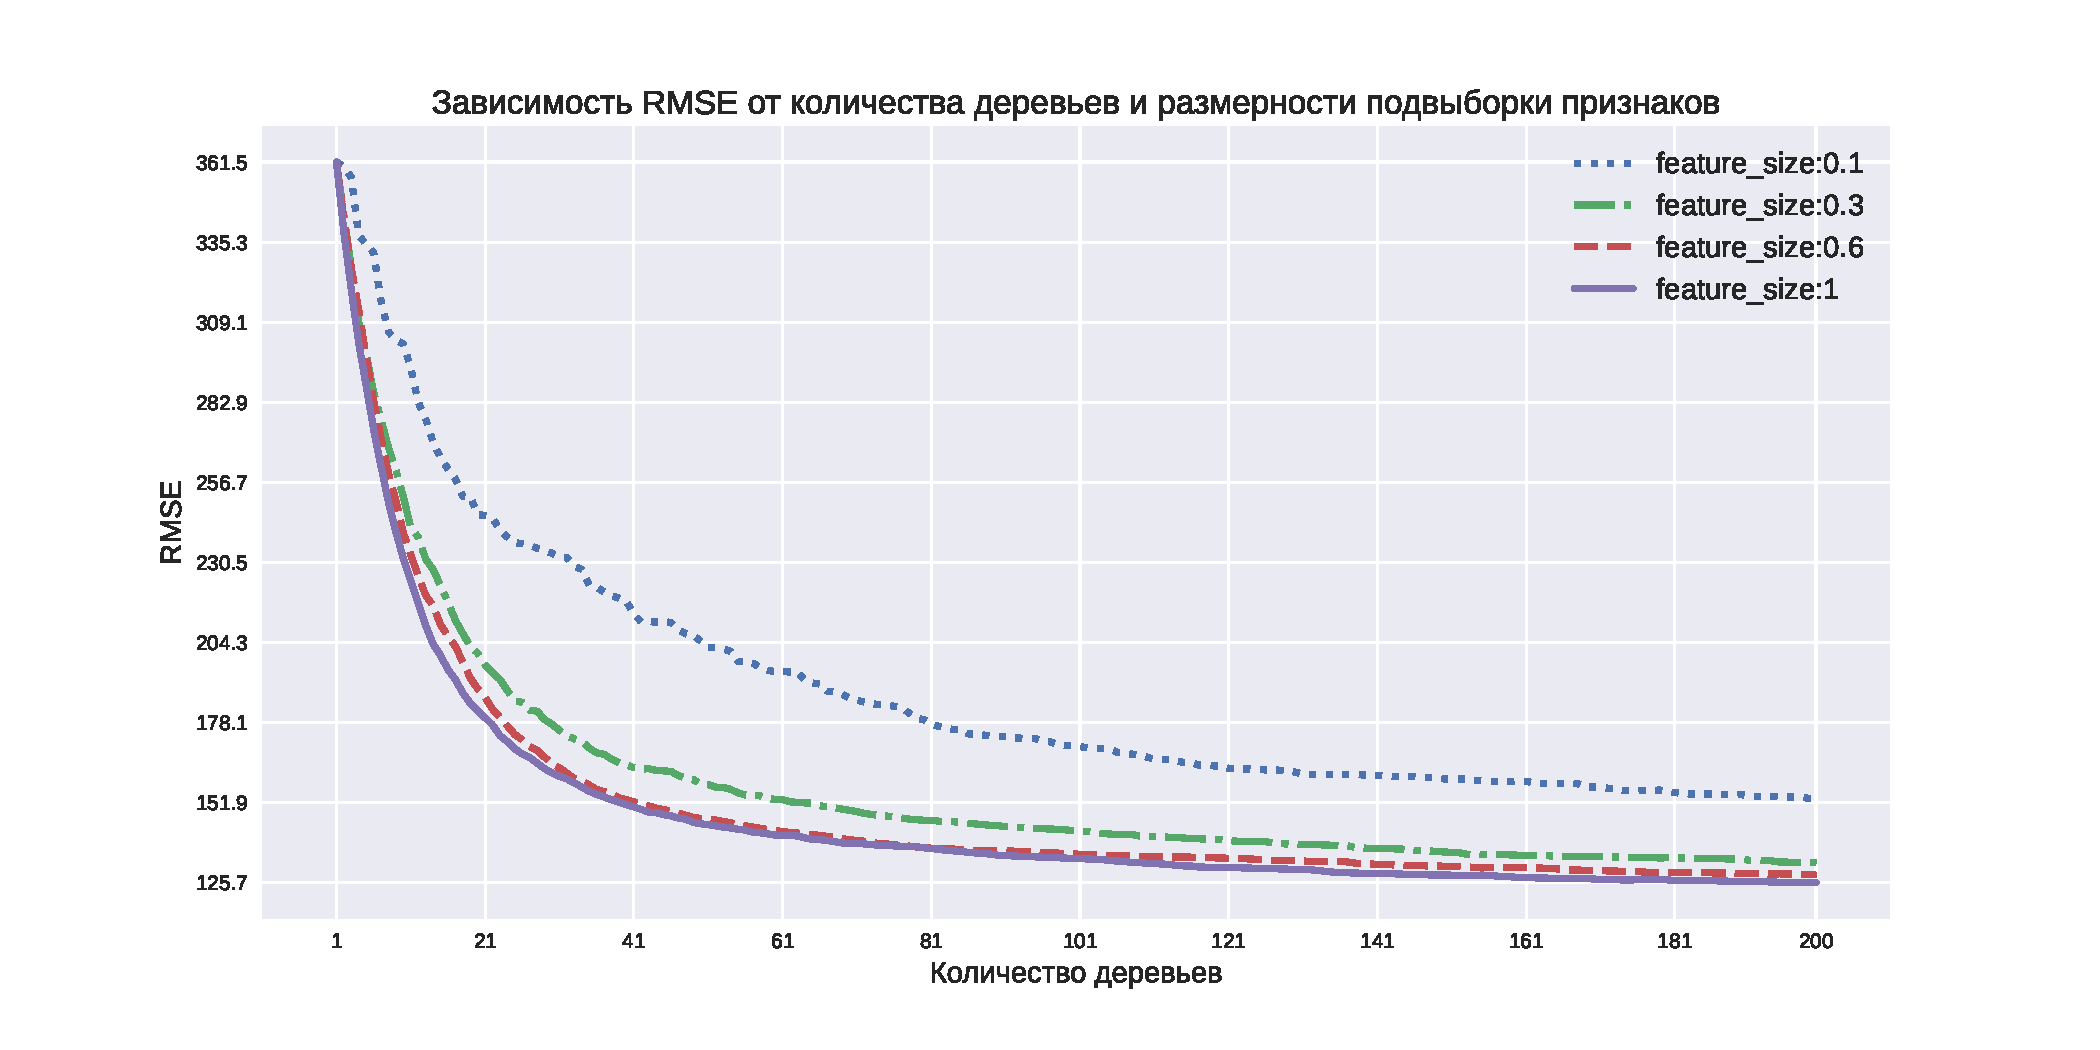
\includegraphics[width=15cm]{31.pdf}
    \caption{Влияние размерности подвыборки на RMSE}
    \label{feature_size_GB}
\end{figure}

На Рис. \ref{feature_size_RF} видно, что лучшее качество получается
при полном наборе признаков для любого количества деревьев в композиции.
Отметим, что чем больше feature\_size, тем лучше качество для данного датасета.
Оптимальное количество деревьев около 150.

\subsection{3.2. Зависимость RMSE от количества и глубины деревьев}

В отличие от RF градиентный бустинг подразумевает построение неглубоких деревьев, чтобы 
каждое следующее дерево исправляло ошибки предыдущих. Поэтому обычно деревья в GB имеют максимальную 
глубину не больше 10.

\begin{figure}[htb]
    \centering
    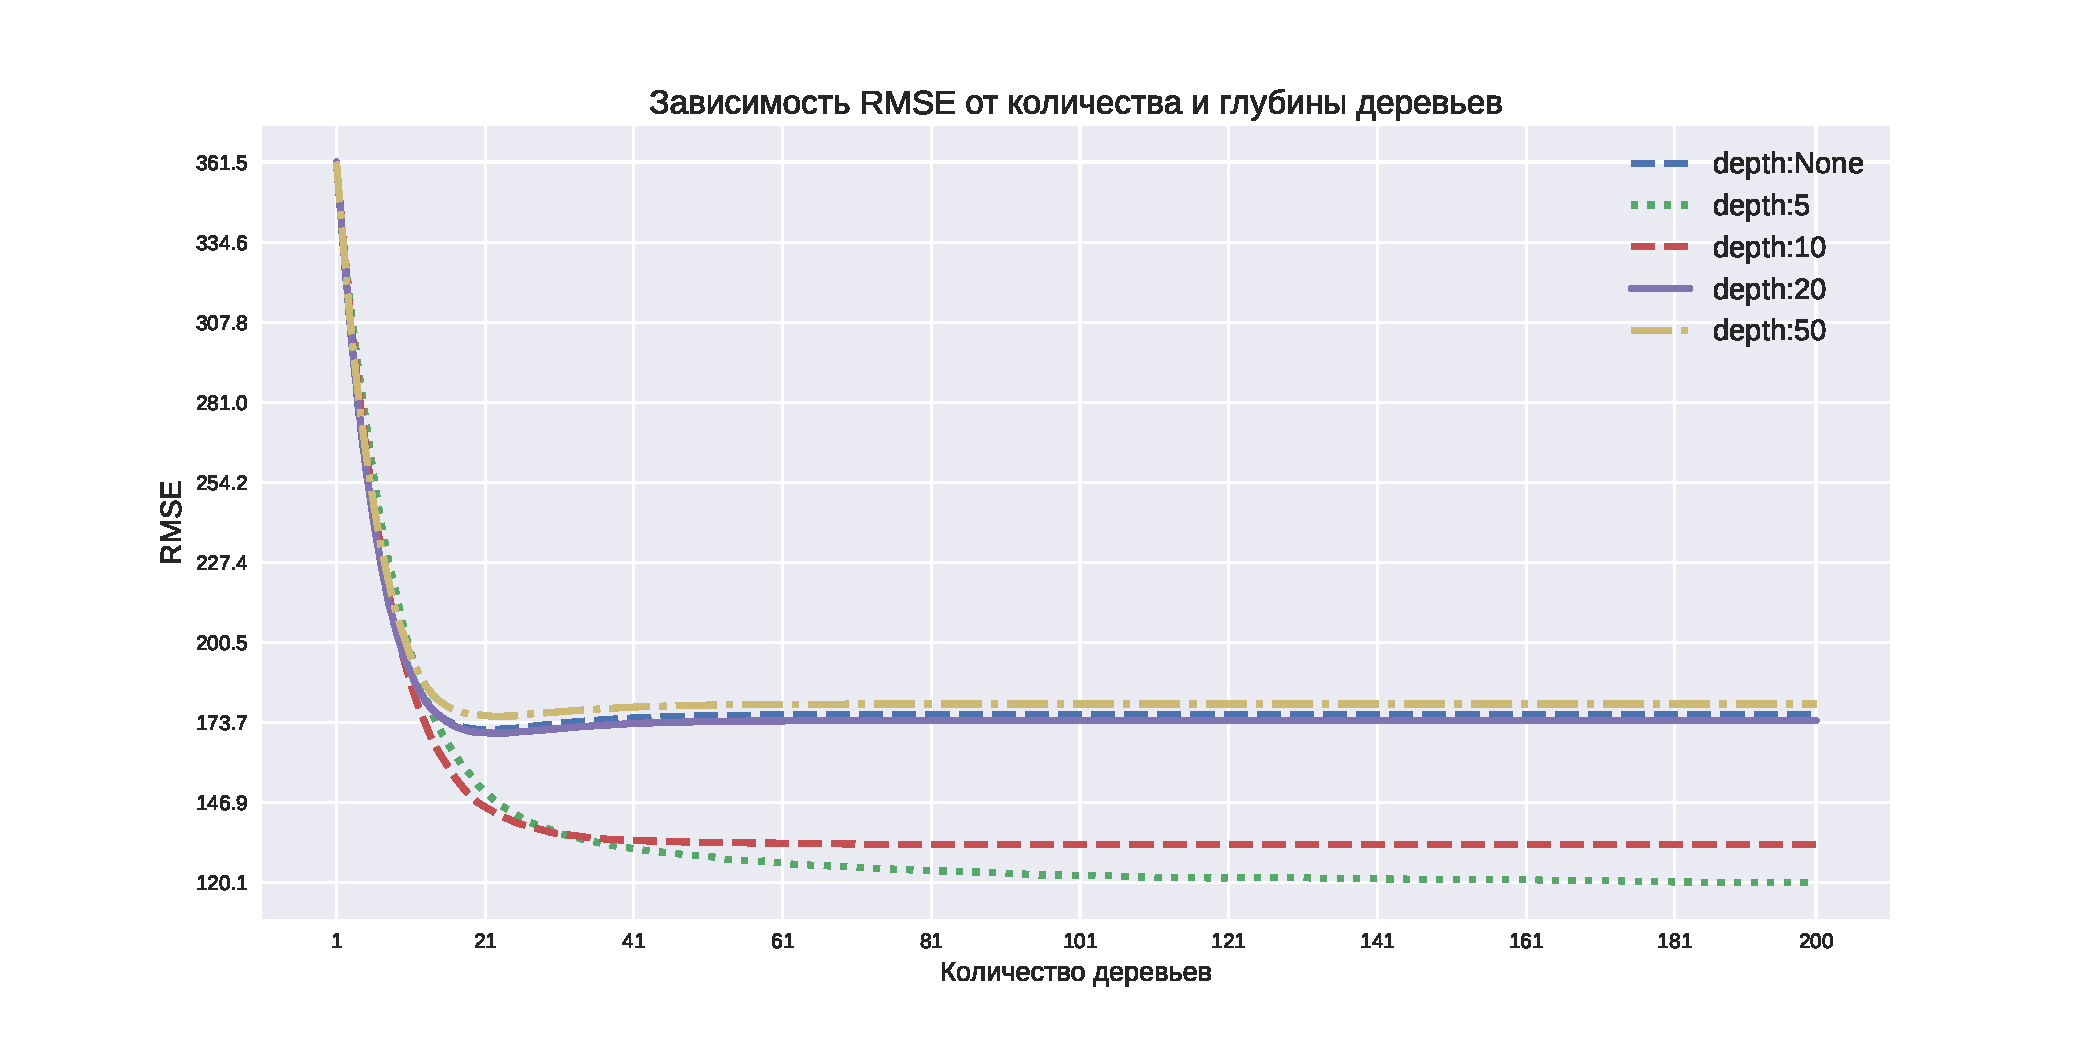
\includegraphics[width=15cm]{32.pdf}
    \caption{Влияние глубины деревьев в композиции}
    \label{depth_GB}
\end{figure}

На Рис. \ref{depth_GB} видно, что лучше всего показали себя алгоритмы с маленькой глубиной.
Алгоритмы с большой/неограниченной глубиной очень быстро выходят на ''плато'' при увеличении количества 
деревьев, причем RMSE заметно больше. Это объясняется тем, что при построении ''мощных''
деревьев в GB в какой-то момент новые деревья перестают быть значимыми, ведь с самого начала 
мы строили деревья, которые пытаются ''объяснить все''\footnote{Очень ненаучно, ну и пусть!}.

\newpage

\subsection{3.3. Зависимость ошибки от скорости обучения}
У градиентного бустинга есть параметр, влияющий на скорость обучения --- learning rate.
Если он будет слишком большим, то алгоритм рискует не сойтись, а если слишком маленьким,
то время на построение алгоритма существенно увеличивается.

\begin{figure}[htb]
    \centering
    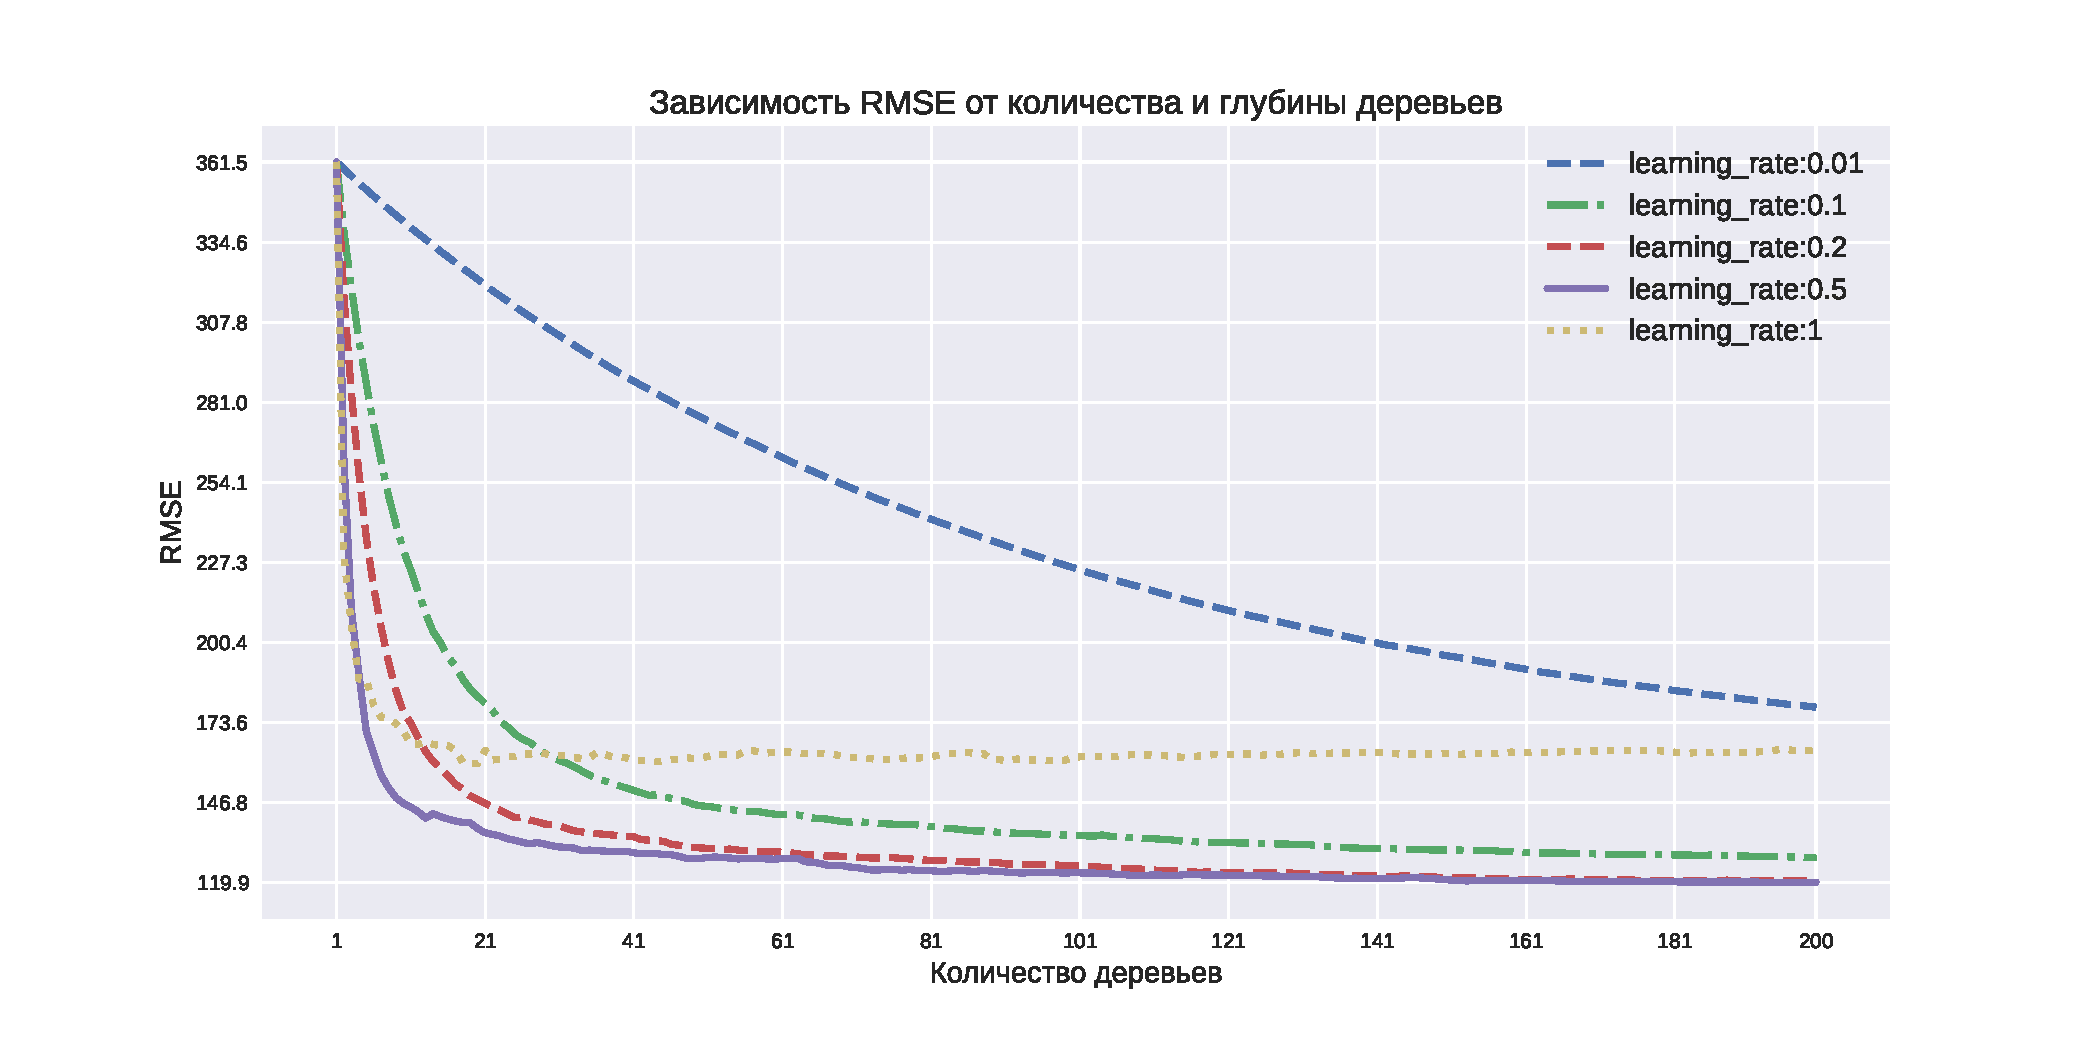
\includegraphics[width=15cm]{33.pdf}
    \caption{Влияние глубины деревьев в композиции}
    \label{rate_GB}
\end{figure}

\noindentОптимальным в данном случае оказалось значение learning\_rate 0.2, 0.5.
\section{Заключение}
\end{document}